\begin{frame}
    \frametitle{Categorical Data Analysis: Cancer Label}
    \begin{itemize}
        \item Analyzing the 'Cancer label' column to identify the most frequent categories.
        \item Using the \textbf{Mode} to determine the most common cancer labels in the dataset.
        \item Visualizing the distribution of cancer labels and their frequencies.
    \end{itemize}
\end{frame}

\begin{frame}[fragile]
    \frametitle{Mode for Categorical Data}
    \begin{itemize}
        \item \textbf{Mode:} The value(s) that appear most frequently in a dataset.
        \item For categorical data, the mode represents the most common category or categories.

        \item \textbf{Interpretation:}
              \begin{itemize}
                  \item The mode cancer labels are the list of numerical values shown above.
                  \item  This output suggests that in the 'Cancer label' column, each unique numerical value appears with the same highest frequency.
                  \item This might indicate that the 'Cancer label' column, as extracted, does not contain typical categorical labels but rather unique numerical identifiers, or that there's an issue with data interpretation.
              \end{itemize}
    \end{itemize}
\end{frame}

\begin{frame}
    \frametitle{Distribution Visualization}
    \begin{itemize}
        \item \textbf{Sorted Bar Graph:} A sorted bar graph was generated to visualize the frequency of each cancer label.
        \item \textbf{Image File:} The graph is saved as \texttt{images/mode.png}.
    \end{itemize}
    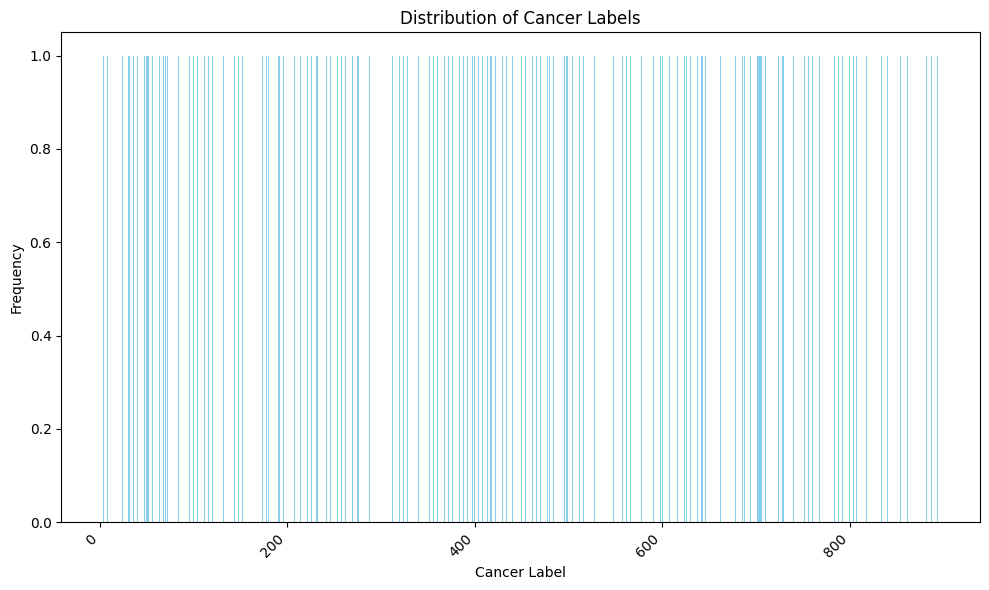
\includegraphics[width=0.8\textwidth]{images/mode.png}
\end{frame}